\documentclass{article}
\usepackage{fontspec}
\usepackage{polyglossia}
\setdefaultlanguage{french}
\usepackage[a4paper,margin=2.5cm]{geometry}

\usepackage{amsmath}
\usepackage{amssymb}
\usepackage{array}
\usepackage{auto-pst-pdf}
\usepackage{booktabs}
\usepackage{cite}
\usepackage{graphicx}
\usepackage{lmodern}
\usepackage{marvosym}
\usepackage{mathrsfs}
\usepackage{minted}
\usepackage{multicol}
\usepackage{multirow}
\usepackage{paralist}
\usepackage{schemabloc}
\usepackage{siunitx}
\usepackage{soul}
\usepackage{tikz}
\usepackage[european,cuteinductors,siunitx]{circuitikz}
\usepackage{url,hyperref}
\usepackage{verbatim}
\usepackage{xunicode,xltxtra}

\title{
\includegraphics{../../../images/inp-enseeiht} \\ ~ \\ ~ \\ ~ \\ ~ \\ Initiation aux outils Silvaco}
\author{François Pierron \& Guilhem Saurel}
\date{\oldstylenums{24 javier 2014}}

\begin{document}

\begin{titlepage}
    \setcounter{page}{0}
    \maketitle
    \vfill
    \tableofcontents
    \thispagestyle{empty}
\end{titlepage}

\section*{Introduction}

Silvaco est une suite logicielle permettant la simulation de processus technologiques sur le dopage et la gravure de semi-conducteurs, puis la simulation électrique de cette simulation physique.

Afin de prendre en main cet outil, nous simulerons un processus NMOS (semblable à ce que nous avons pu faire en salle blanche), si jamais nous arrivons à comprendre cette étrange logique qui consiste à utiliser le clic droit pour ouvrir un menu.

\section{Athena}

Athéna est l’outil de simulation de processus technologique. L’utiliser consiste à lui indiquer les différentes actions à effectuer sur le substrat lors des différentes étapes de la fabrication.
Ces étapes sont à écrire simplement les unes à la suite des autres dans un fichier texte ; mais heureusement pour chaque type d’action une interface graphique nous permet de générer les lignes correspondantes dans ce fichier texte, lorsque nous ne connaissons pas encore parfaitement la syntaxe.

\subsection{Étape 0: Définition du mesh et du substrat}
Cette première étape n’est pas véritablement une étape du processus technologique, mais permet d’indiquer au logiciel les différents points où il faudra qu’il effectue les calculs.
Cette étape est primordiale, puisque plus le maillage sera fin, plus les calculs seront précis, mais plus le temps de calcul sera élevé.

Vu que ce NMOS est symétrique, nous allons seulement simuler la création d’une moitiée de transitor, puis nous effectuerons un miroir sur cette moitié.

~

L’idée lors de la création de cette grille est de mettre un maillage fin aux endroits importants, tels que les interfaces entre les différentes zones, et une grille plus grossière lorsque l’on se trouve dans des zone homogènes.

\inputminted[linenos,lastline=17]{sh}{final_named.in}

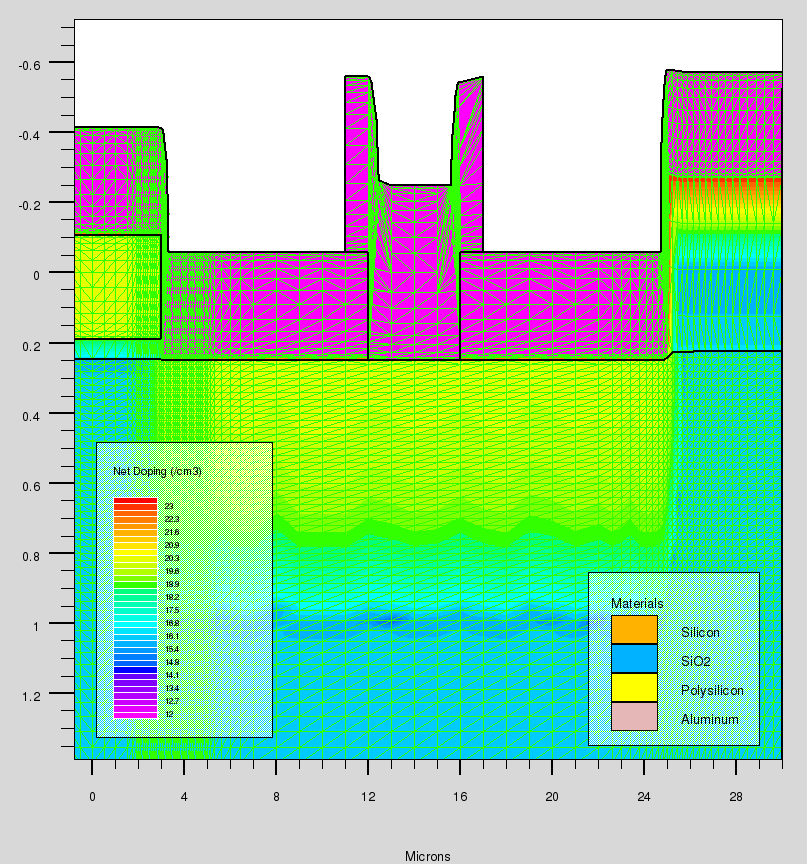
\includegraphics[width=\linewidth]{mesh.png}

Cette capture a été prise à la fin du projet, afin qu’on comprenne pourquoi le mesh est plus dense à certains endroits qu’à d’autres. Aussi, pour l’instant, la simulation et TonyPlot ne considèrent qu’une dimension.

~

Pour la définition du substrat, nous utiliserons un silicium dopé au Bore à $10^{16}$ cm$^{-3}$, qui a une orientation <100>:
\inputminted[linenos,firstnumber=18,firstline=18,lastline=19]{sh}{final_named.in}

\subsection{Étape 1: Croissance de l’oxyde de champ}
Cette étape correspond au premier passage dans le four, où l’on simule une montée en température, l’addtion d’oxygène et d’hydrogène pendant différentes durées puis une redescente en température

\inputminted[linenos,firstnumber=20,firstline=20,lastline=30]{sh}{final_named.in}

Ensuite, pour mesurer l’épaisseur d’oxyde, il y a une commande:
\inputminted[linenos,firstnumber=31,firstline=31,lastline=32]{sh}{final_named.in}

Ce qui nous donne une épaisseur d’oxyde de 0.4905µm, ce qui est très proche de l’épaisseur obtenue en salle blanche (0.4932µm).

Puis on peut sauvegarder les resultats de la simulation dans un fichier str:
\inputminted[linenos,firstnumber=33,firstline=33,lastline=33]{sh}{final_named.in}

(Par lu suite, nous aurons de multiples sauvegardes telle que celle-ci, mais il n’est pas pertinent de toute les décrire…)

\subsection{Étape 2: Ouverture de la zone active}
Pour ouvrir la zone active afin de permettre le dopage de la source ou du drain, et d’avoir une épaisseur d’oxyde moindre pour la grille, il suffit de graver au bon endroit:
\inputminted[linenos,firstnumber=34,firstline=34,lastline=36]{sh}{final_named.in}

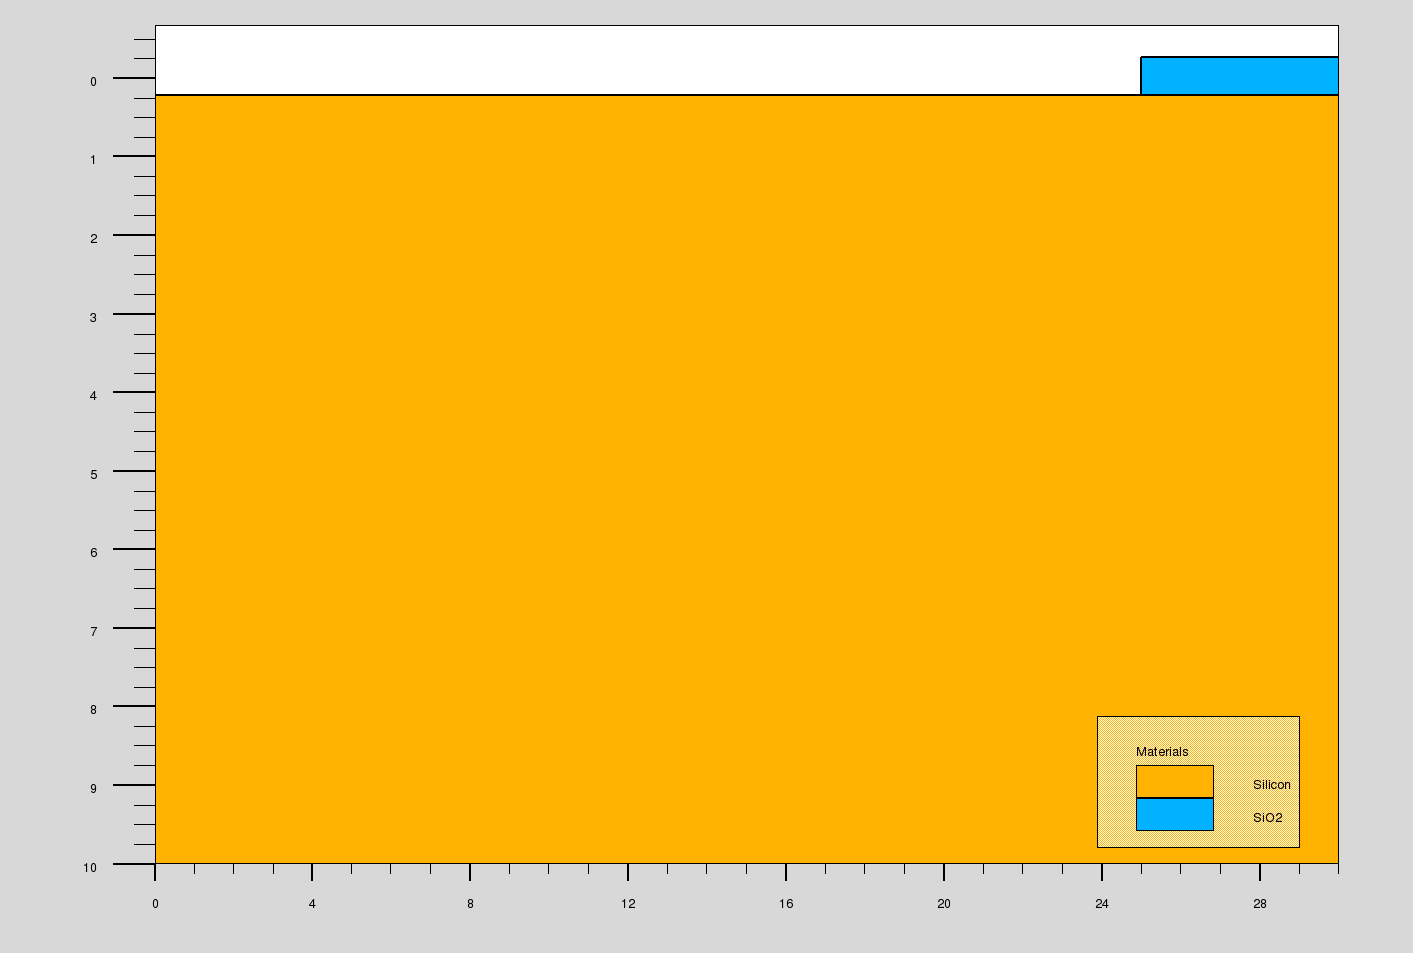
\includegraphics[width=\linewidth]{1ouverture.png}


\subsection{Étape 3: Croissance de l’oxyde de grille}
Une fois que nous sommes revenu au silicium non oxydé à l’endroit où se trouvera la grille, il nous faut ajouter une mince couche d’oxyde avant le dépôt de polysilicium:
\inputminted[linenos,firstnumber=37,firstline=37,lastline=42]{sh}{final_named.in}

On peut alors mesurer l’épaisseur de cet oxyde:
\inputminted[linenos,firstnumber=43,firstline=43,lastline=47]{sh}{final_named.in}

Ce qui donne 0.0564 µm, ce qui s’approche de la théorie à 0.045µm et de la pratique en salle blanche à environ 0.075µm.

On peut également mesurer l’épaisseur de silicium qui a disparu pour s’oxyder : $0.22207-0.24681=0.02474$ µm.

On peut donc comparer cette valeur avec les résultats théoriques, qui disent que l’épaisseur de silicium ayant disparu correspond à 44\% de l’épaisseur d’oxyde finale : $\cfrac{0.02474}{44 \%} = 0.0562 \simeq 0.0564$ ; on est donc très proche de cette théorie.

On remarque que la durée d’éxécution de cette commande est effectivement plus longue que clle de l’étape 1 ; la différence est que lors de l’étape 1 l’une des deux dimensions ne variait pas du tout, alors qu’ici, puisque nous avons ouvert 25µm, un calcul en deux dimensions est indispensable.

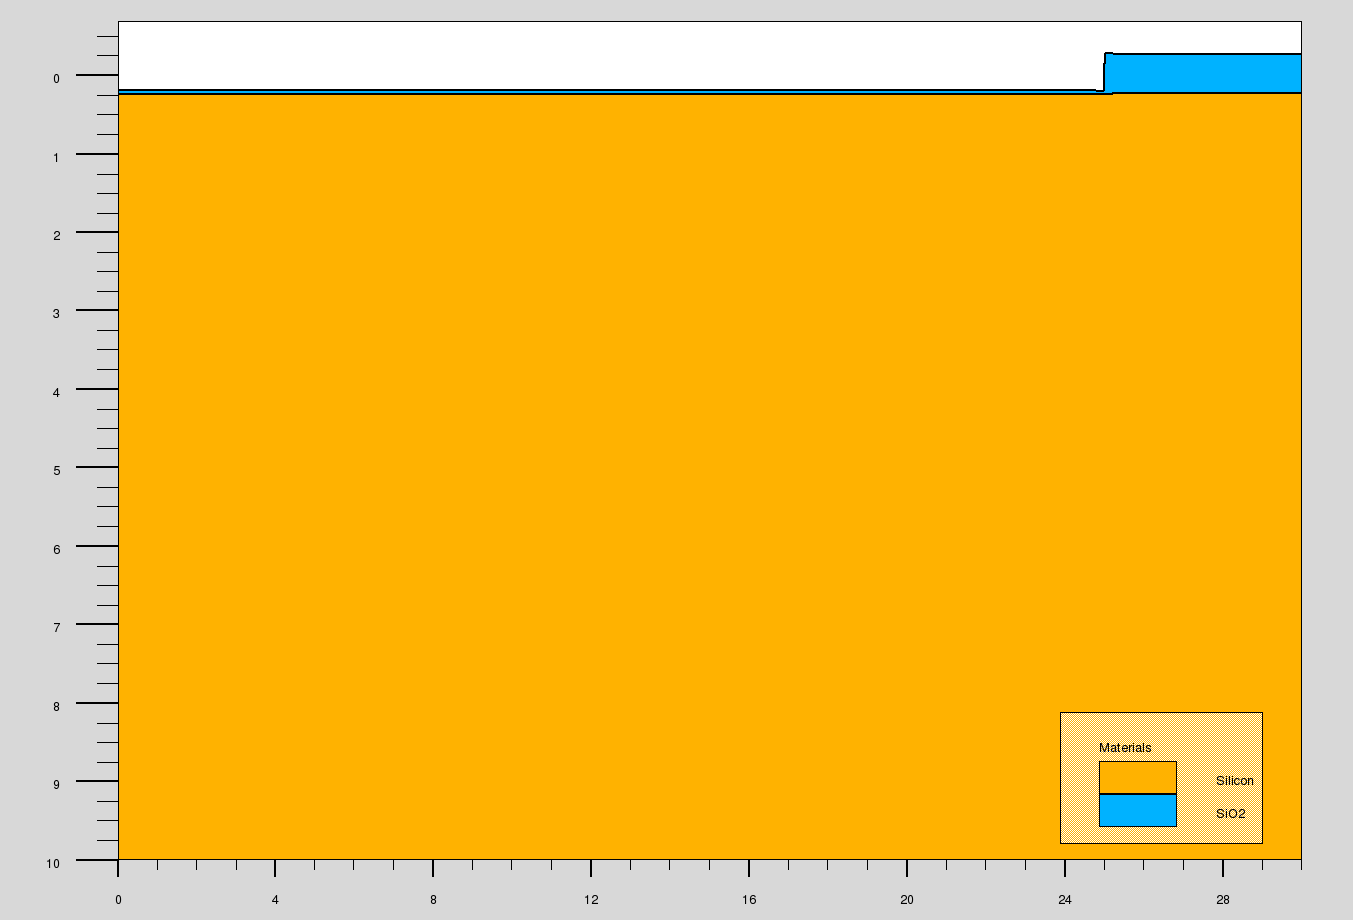
\includegraphics[width=\linewidth]{3_gate_oxy.png}

\subsection{Étape 4: Dépôt de polysilicium}
L’étape suivante consiste à déposer le polysilicium qui servira de «métal» pour la grille:
\inputminted[linenos,firstnumber=48,firstline=48,lastline=50]{sh}{final_named.in}

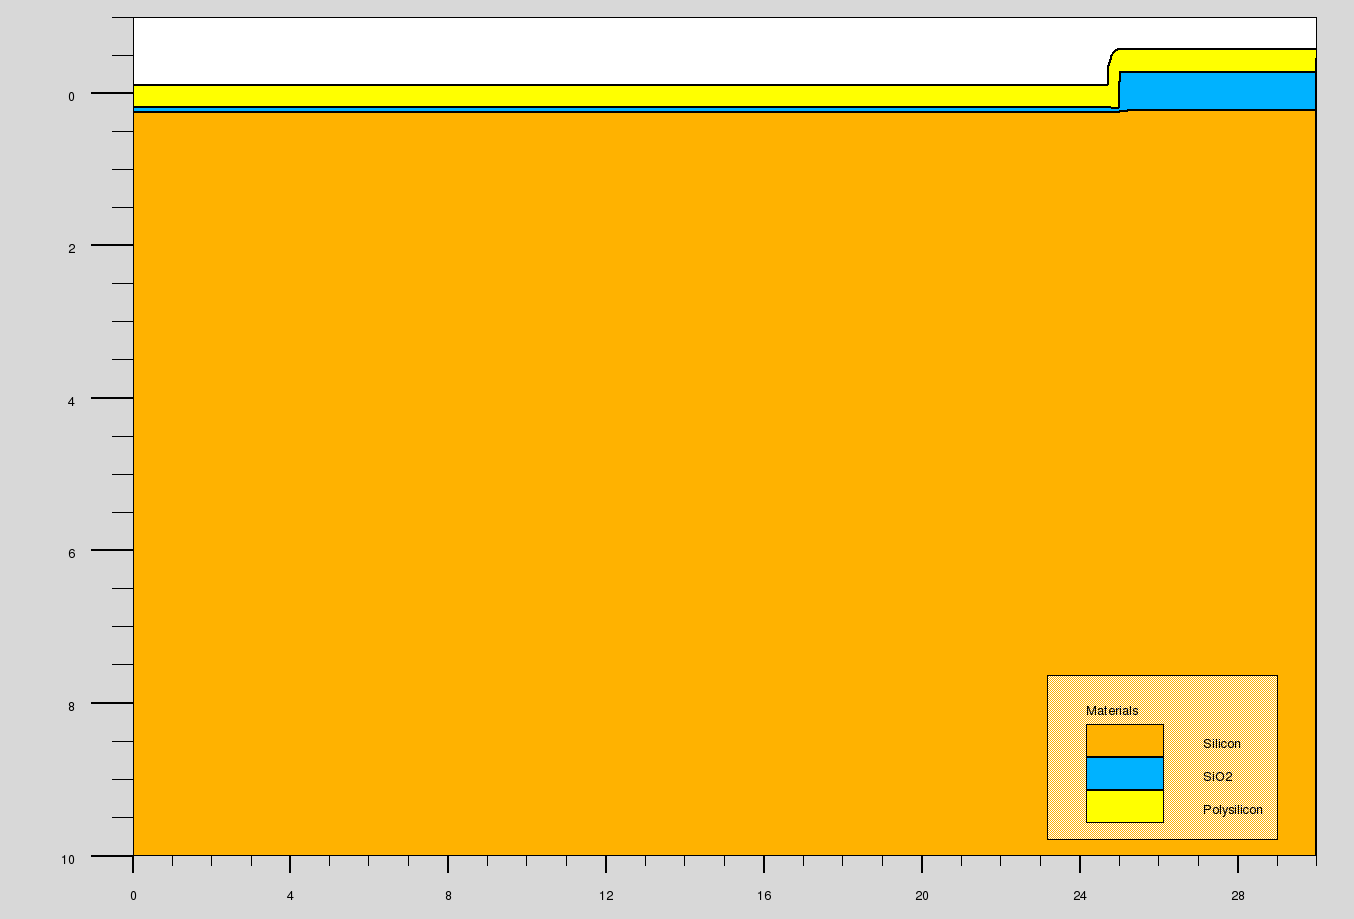
\includegraphics[width=\linewidth]{4_poly.png}

\subsection{Étape 5: Gravure du polysilicium et de l’oxyde de grille}

Pour la gravure du polysilicium, pas spécialement de surprise:
\inputminted[linenos,firstnumber=51,firstline=51,lastline=52]{sh}{final_named.in}

Par contre, pour la gravure de l’oxyde de grille, il faut définir un rectangle, afin de ne pas toucher à l’oxyde de champ:
\inputminted[linenos,firstnumber=53,firstline=53,lastline=60]{sh}{final_named.in}

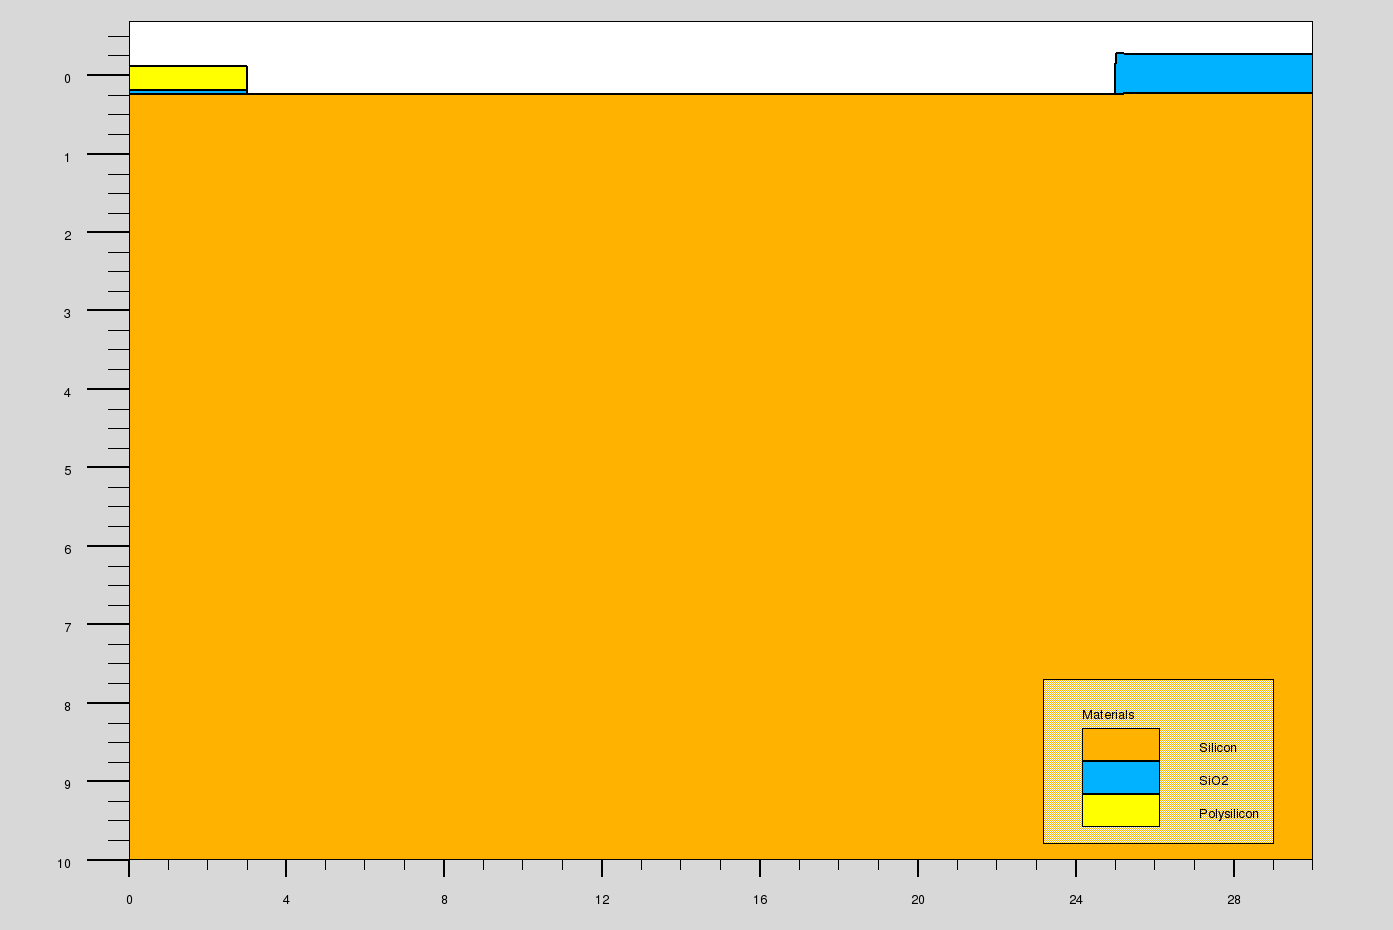
\includegraphics[width=\linewidth]{5gate.png}

\subsection{Étape 6: Pré-dépôt de phosphore}

Encore un passage dans le four, où l’on ajoute cette fois du phosphore afin de réaliser le dopage des sources et des drains du transistor:
\inputminted[linenos,firstnumber=61,firstline=61,lastline=69]{sh}{final_named.in}

On peut alors utiliser l’outil TonyPlot pour mesurer la dose de ce phosphore dans notre wafer, et nous avons $2.15\cdot10^{20}$ cm$^{-2}$ en intégrant la concentration du dopage sur une section verticale.

\subsection{Étape 7: Redistribution}
Cette étape est un «recuit» de notre wafer afin de l’uniformiser, et de «réparer» la structure cristalline du silicium ayant souffert lors du passage des atomes de phosphore, qui sont beaucoup plus gros que ceux de silicium. Cela permet égalemement à ces atomes de phosphore de pénétrer un peu plus dans le silicium pour augmenter la profondeur de jonction, mais cela entraine qu’ils pénétrent également un peu plus profondément sous la grille, ce qui va donc modifier sa longueur effective.

\inputminted[linenos,firstnumber=70,firstline=70,lastline=74]{sh}{final_named.in}

On mesure alors une demi-longueur effective de grille de 2.5µm, au lieu de 3µm.

Si l’on mesure à nouveau la dose de phosphore, on trouve $2.14\cdot10^{20}$ cm$^{-2}$. Cette différence ne s’explique évidement pas parce que du phosphore a disparu, mais simplement parce qu’une partie du phosphore est parti sous la grille, et que donc le nombre total d’atome s’est étiré en largeur, ce qui entraine que sur une coupe verticale, la concentration est moindre.

Aussi, peut être que sur d’autres coupes verticales, la concentration était inférieure, et que lors de l’uniformisation tout ceci a convergé vers une moyenne.

D’ailleurs, il est intéressant de noter à ce niveau que si l’on ne fait pas la coupe verticale exactement au même endroit que la simulation précédente, nous obtenons des résultats aléatoires voir aberrants, comme un dopage multiplié par deux en cours de route. C’est tout à fait logique, puisque le logiciel simule les imperfections de l’uniformité des différentes étapes.

Nous mesurons la profondeur de jonction qui était à 0.754µm, ce qui reste relativement proche de celle obtenue en salle blanche (1.15µm).

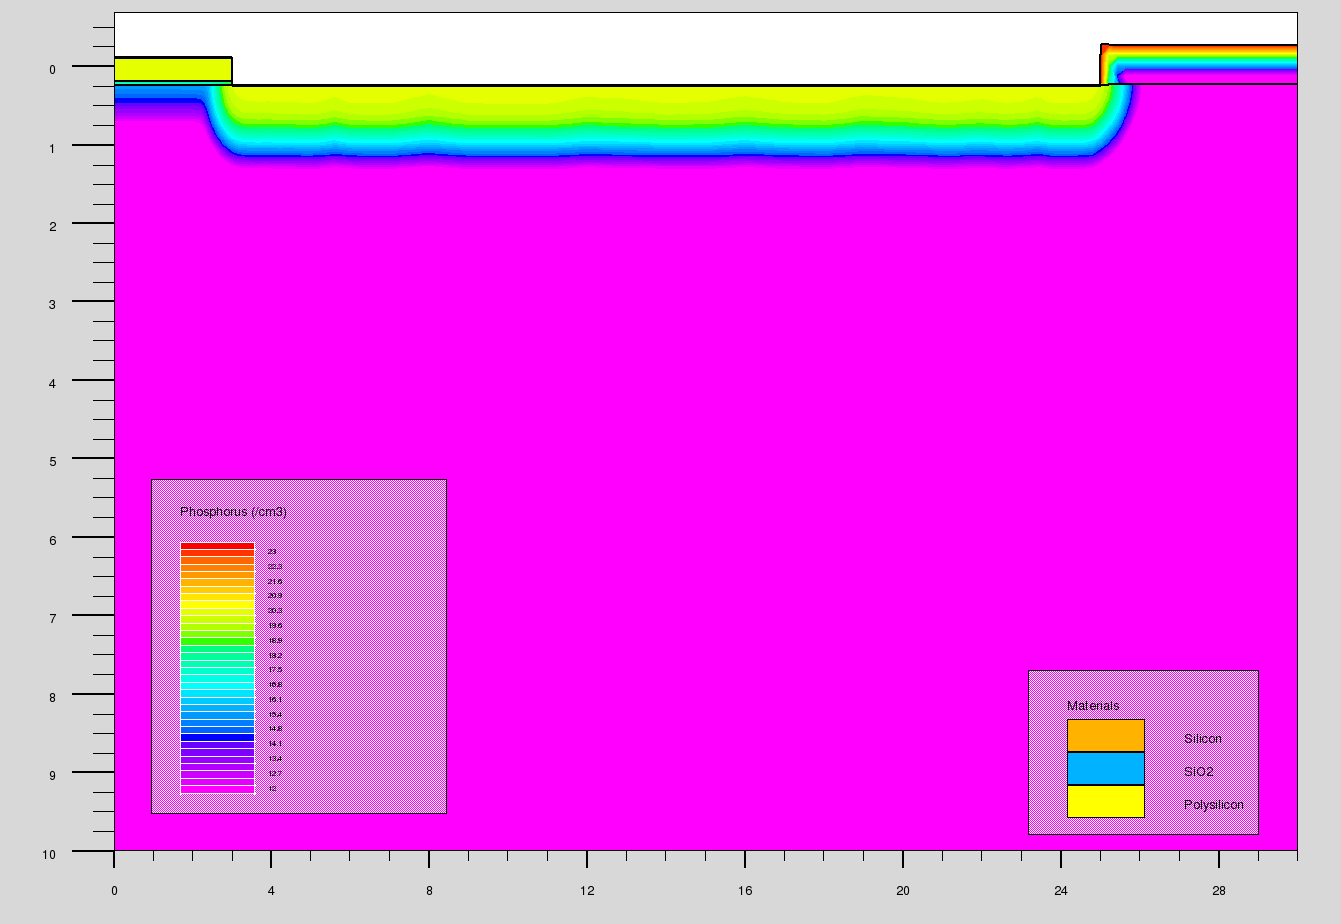
\includegraphics[width=\linewidth]{7_dopage.png}

\subsection{Étape 8: Oxydation à basse température (LTO)}
Avant d’ajouter le métal, il vaut mieux mettre une couche d’isolant où l’on ne veut pas qu’il y ait contact. C’est le but de cette nouvelle étape d’oxydation.

\inputminted[linenos,firstnumber=75,firstline=75,lastline=79]{sh}{final_named.in}

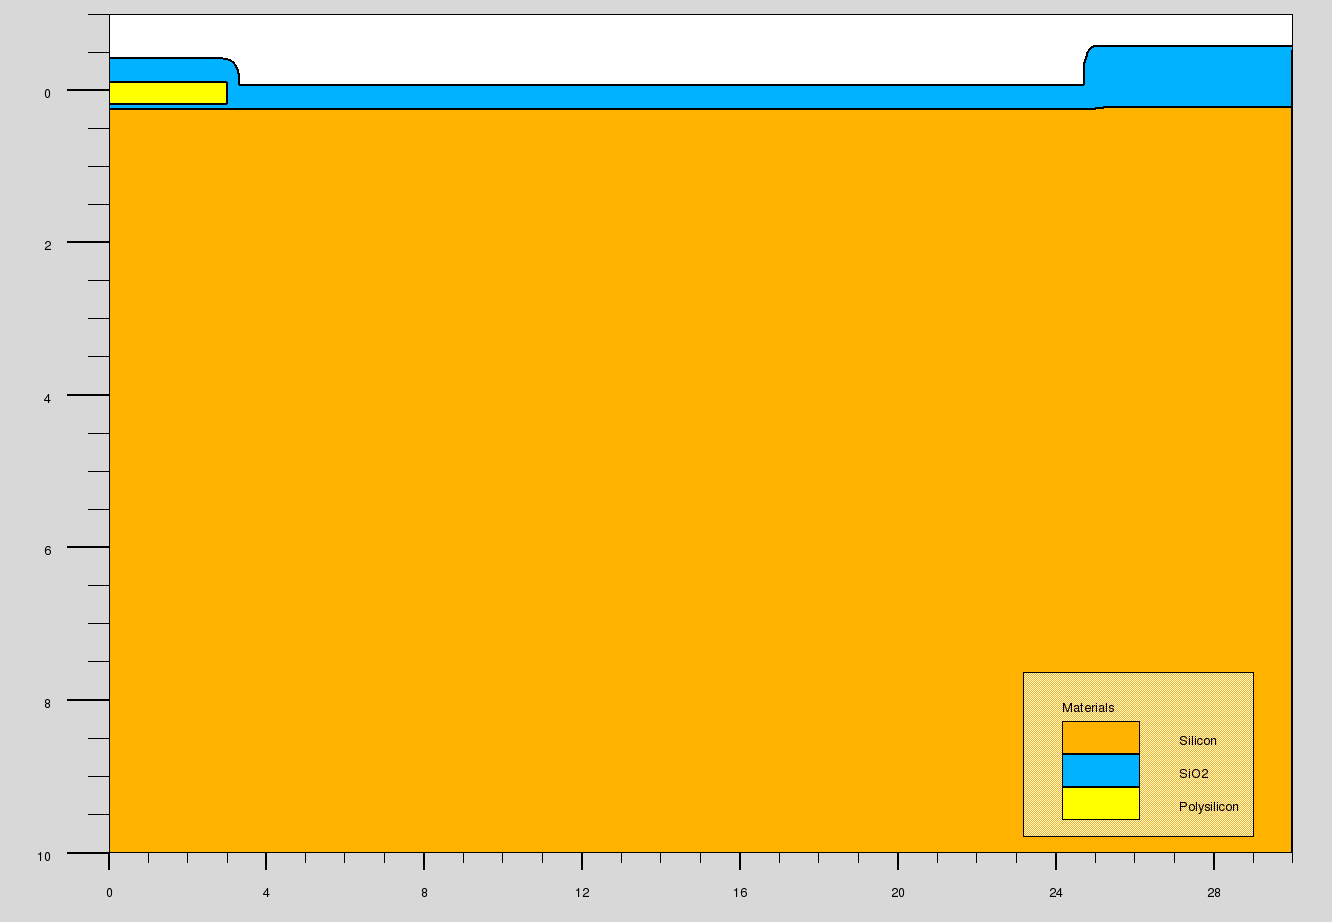
\includegraphics[width=\linewidth]{8croissance_oxide.png}

\subsection{Étape 9: Ouverture des contacts}

Le drain (et donc la source) sont maintenant recouverts d’oxyde, mais il faut bien l’ouvrir à l’endroit où l’on veut un contact avec le métal:
\inputminted[linenos,firstnumber=80,firstline=80,lastline=86]{sh}{final_named.in}

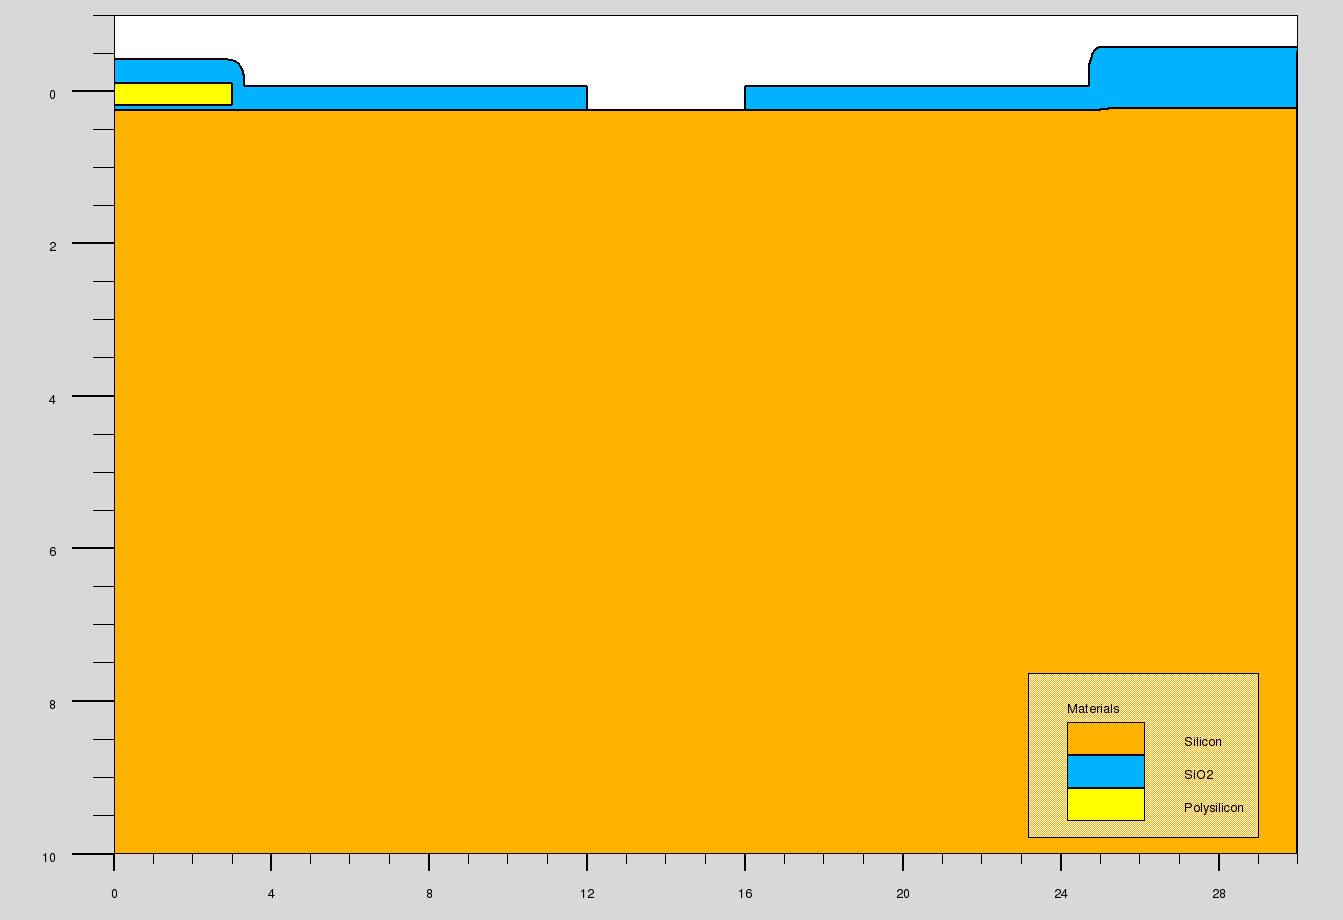
\includegraphics[width=\linewidth]{9_via.png}

\subsection{Étape 10: Métalisation et gravure}
On va enfin pouvoir ajouter nos contacts. Pour cela, on recouvre tout le wafer d’aluminium, puis on le grave afin de ne garder que ce qu’il y a au niveau du drain et de la source:
\inputminted[linenos,firstnumber=87,firstline=87,lastline=97]{sh}{final_named.in}

(Cette capture ne rend pas compte de la gravure, mais uniquement du dépôt d’aluminium).

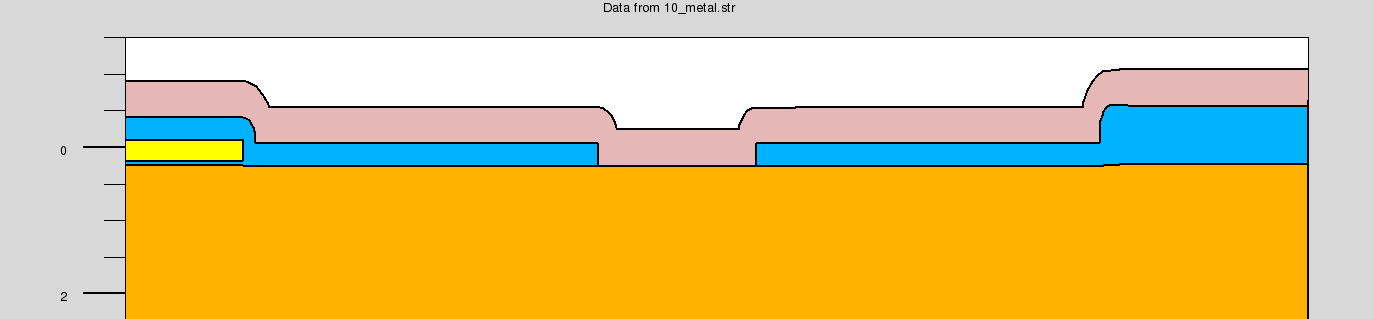
\includegraphics[width=\linewidth]{10_depot_metal.png}

\subsection{Étape 11: Finitions}
Cette étape est à nouveau une étape qui ne correspond pas vraiment à une étape technologique, mais il nous faut créer un miroir vertical de notre structure puisque jusque là nous n’en avions que la moitié, et il faut indiquer au logiciel où sont le drain, la source, la grille et le substrat.

Bien sûr, nous n’avons pas créé de contact métallique au niveau de la grille, comme nous l’avons fait pour le drain et la source, puisqu’il ne faut en aucun cas ajouter de métal au-dessus de la grille au niveau de l’effet transistor.

\inputminted[linenos,firstnumber=98,firstline=98]{sh}{final_named.in}

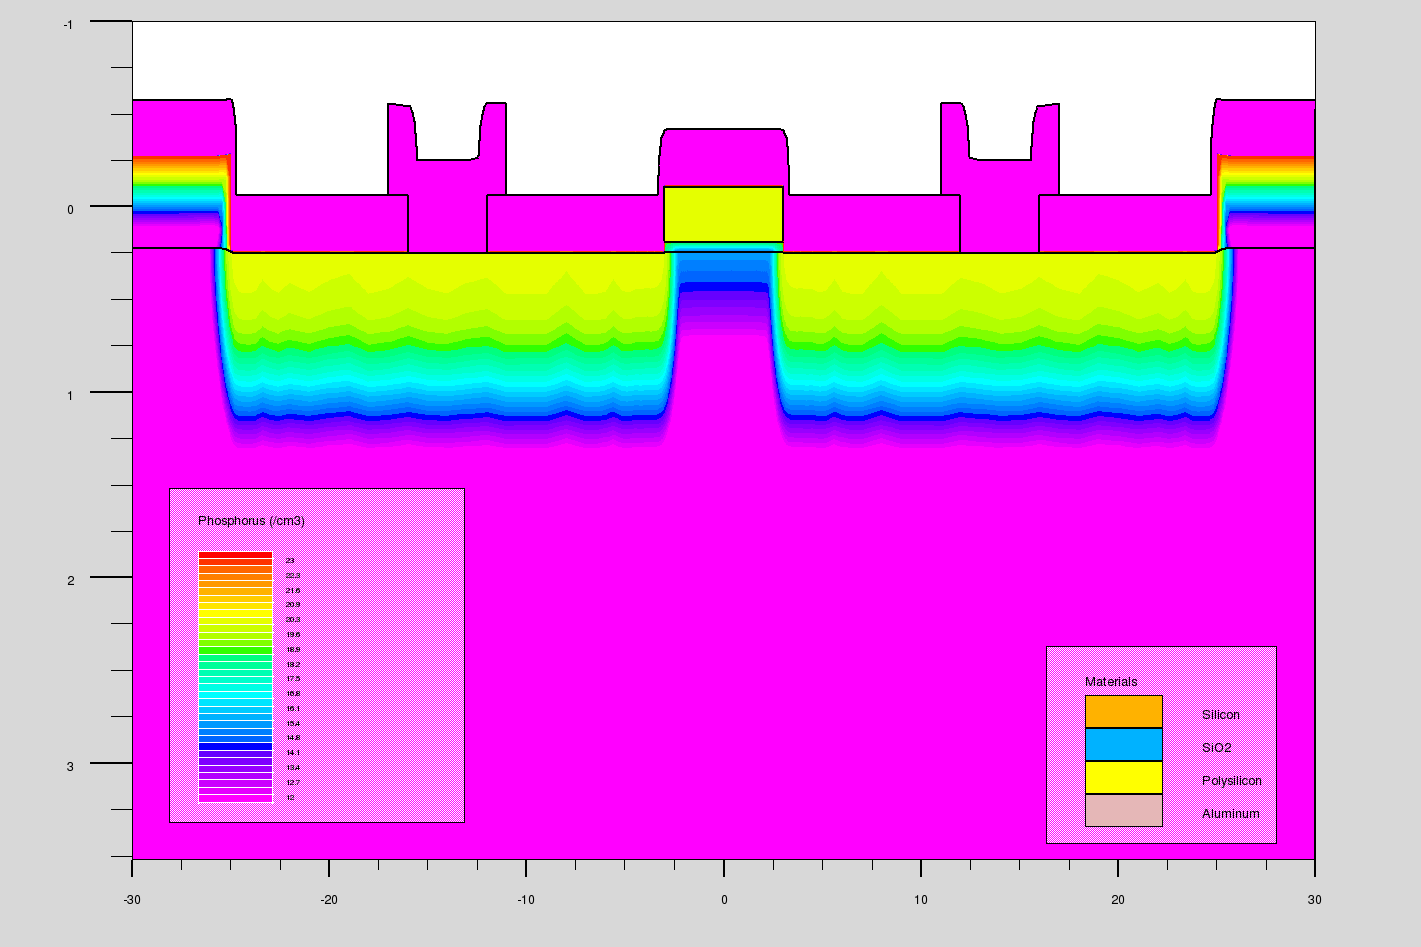
\includegraphics[width=\linewidth]{final.png}

\section{Atlas}

Une fois que nous avons simulé la fabrication de notre MOS, il ne reste plus qu’à tracer ses charactéristiques.

Il faut pour cela utiliser Atlas, et vérifier que le nombre de points sur lesquels on va effectuer les calculs n’est pas trop important, car la simulation prendrait des jours.

\subsection{Détermination de la tension de seuil}

Une fois cette simulation effectuée, on peut tracer $I_{ds}=f(V_{gs})$:

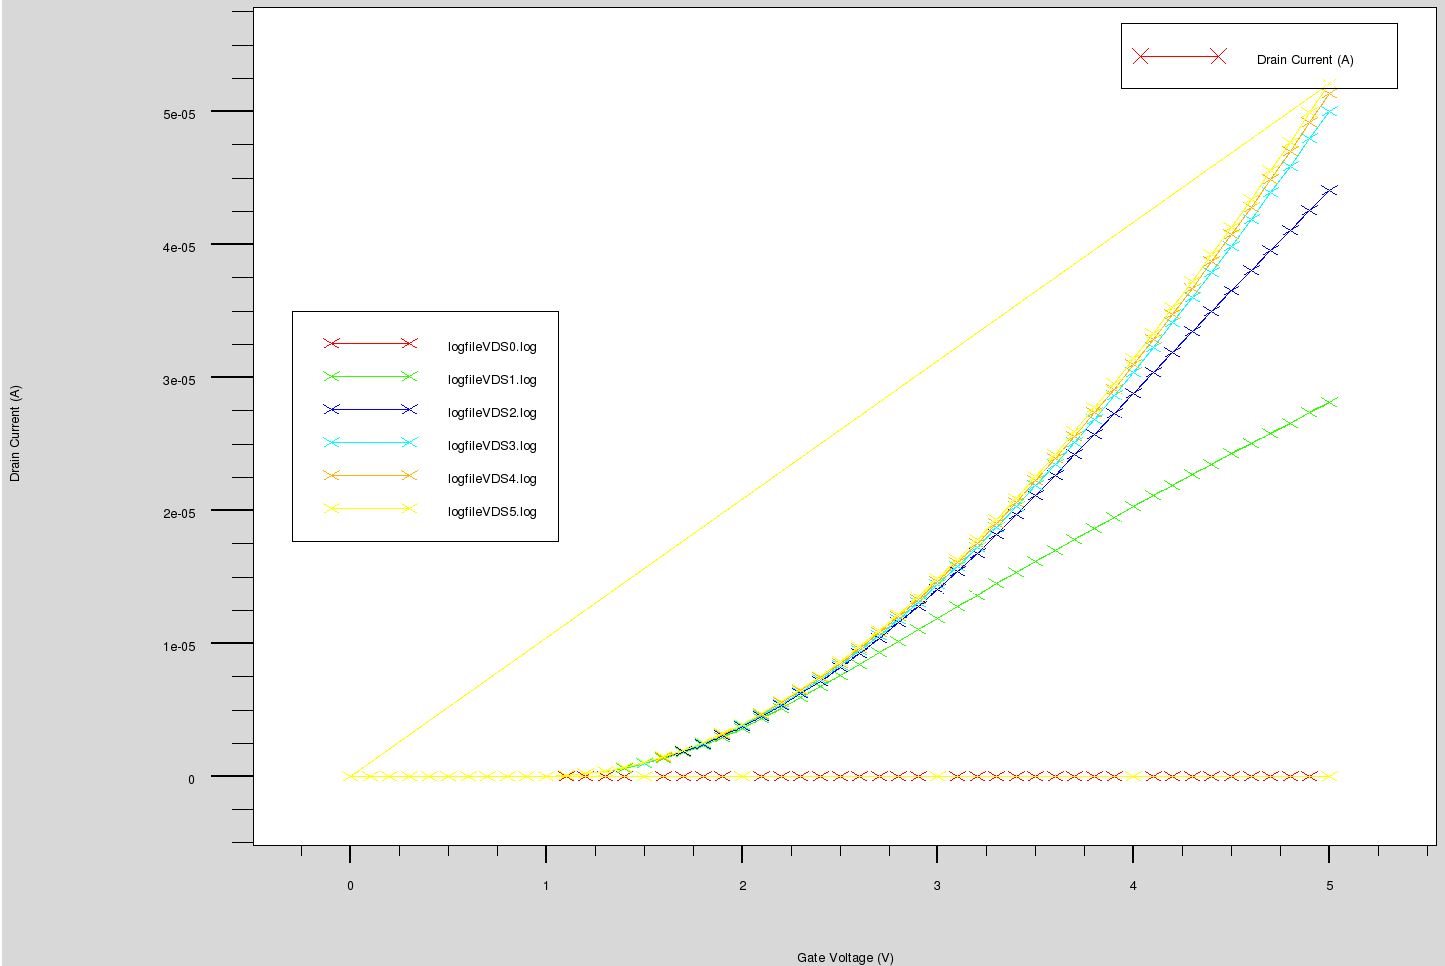
\includegraphics[width=\linewidth]{Id_f_de_VG_pour5_VD.png}

On peut donc mesurer sur cette courbe la tension de seuil ($\simeq2$V) ainsi que la transconductance ($1.7\cdot10^{-5}\Omega^{-1}$).

\subsection{Charactéristique}

De la même manière, on peut tracer la charactéristique $I_{ds}=f(V_{ds})$ pour différents $V_{gs}$:

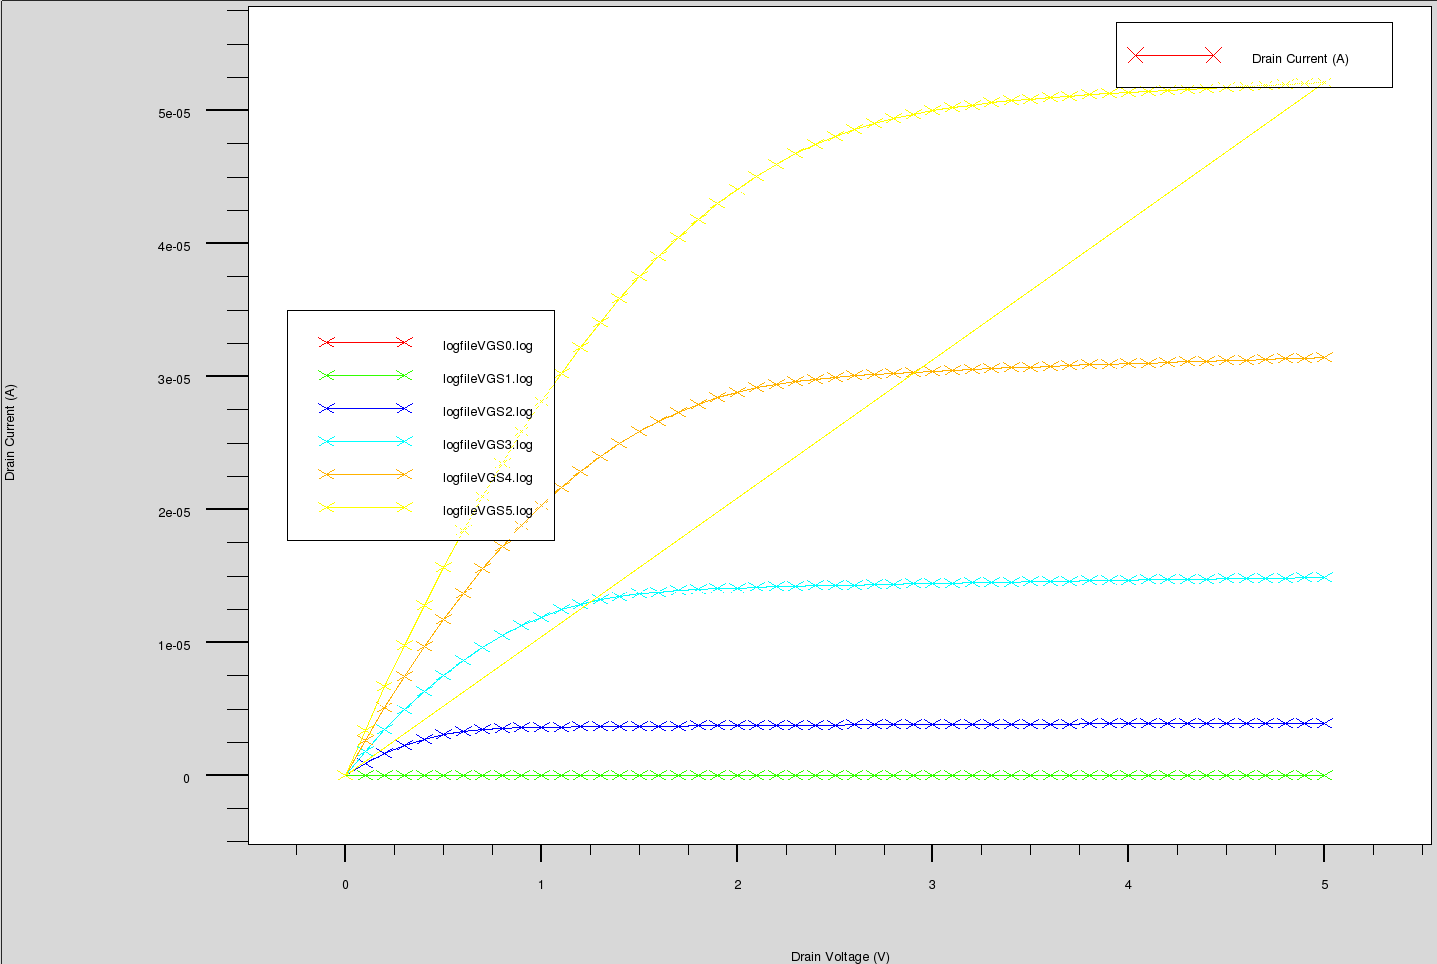
\includegraphics[width=\linewidth]{Id_f_de_VD_pour5VG.png}

On peut alors mesurer la conductance dans la zone ohmique ($3\cdot10^{-5}\Omega^{-1}$ pour un $V_{gs}$ de 5V), et observer que la courbe correspondant à un $V_{gs}$ de 2V est la première à avoir un courant non nul.

\section*{Conclusion}

Malgré certains comportements étranges de son interface (comme un bouton «OK» d’une fenêtre de création d’une coupe verticale qui ne crée pas la coupe verticale), ce logiciel nous a permis de revoir toutes les étapes du processus technologique de création d’un transistor MOS en les simulant, et à vérifier les différents réltats que nous avions pu mesurer lors de notre semaine passée en salle blanche.

\end{document}
